\documentclass{article}
\usepackage[utf8]{inputenc}
\usepackage{graphicx}
\usepackage{hyperref}
\usepackage{listings}
\setlength{\oddsidemargin}{0in}
\setlength{\evensidemargin}{0in}
\setlength{\textheight}{9in}
\setlength{\textwidth}{6.5in}
\setlength{\topmargin}{-0.5in}

\title{122B Spring 2016 \\ Program 2}
\author{Russell Miller and Rylan Schaeffer }

\begin{document}

\maketitle

\section*{Introduction}
\indent \indent Quicksort, quickselect and deterministicselect are three algorithms that can be used to select the $k$th smallest element of an unordered list. We compared their relative performance (measured by time to correct result) as a function of the length of the list. To do so, we analyzed the algorithms and gathered experimental data from randomly generated lists to confirm our analysis. We conclude that although the performances of the three algoriths are comparable for shorter lists, the performances begin to differ for longer lists, with quickselect emerging as the clear winner.

\section*{Algorithm Analysis}
\subsection*{Quickselect}
\indent \indent Quickselect finds the $k$th smallest element of the list by choosing an element from the list (called the pivot) and then partitions the list into elements less than the pivot and elements greater than the pivot. Having done so, the pivot is in its final location between the two partitions. If we call the index of the pivot $p$, we recurse into the left side if $k < p$ or recurse into the right side if $k > p$. This divide-and-conquer strategy can perform well on average, but can also perform poorly in the worst case. Quickselects performance depends on the ``goodness" of the pivot. If a pivot is chosen so that the other elements are split evenly (or almost evenly) on either side of the pivot, the search space decreases by half and the runtime is linear i.e. $O(n)$. But if a pivot is chosen so that the other elements are placed entirely (or almost entirely) on one side of the pivot, the search space barely decreases and the runtime is quadratic i.e. $O(n^2)$.



\subsection*{Deterministicselect}
\indent \indent Deterministicselect is a modified version of quickselect that cleverly chooses the pivot to be the median (or near the median, more precisely) of the list; by doing so, the list partitions are guaranteed to be approximately the same length and thus the worst-case runtime is $O(n)$. To select a pivot value near the median, deterministicselect splits the list into small groups (in our implementation, groups of 5 or fewer), computes the median of each group, and then repeats recursively until only one value remains. At this point, a pivot has been selected and deterministicselect proceeds in a manner identical to quickselect. To understand why the worst-case runtime is $O(n)$, let $T(n)$ be the time to select the kth smallest number. Since the list is divided into $\frac{n}{5}$ groups and the pivot is selected as the median of the groups' medians, $T(\frac{n}{5})$ time is required to determine the median. Then, to partition the list elements on either side of the pivot requires $O(n)$ time. Finally, in the worst case, the pivot was selected so that 70\% of the list's elements fall on the side of the pivot that will be recursed into, requiring $T(\frac{7n}{10})$ time. Thus, $$T(n) \leq T(\frac{n}{5}) + n + T(\frac{7n}{10})$$

Applying the Master Theorem tells us that the runtime will be worst-case $O(n)$.

\subsection*{Quicksort}
\indent \indent Quicksort differs from the two prior algorithms in that quicksort is a sorting algorithm; that is, quicksort rearranges all elements of the list in increasing order. To select the $kth$ smallest element, one simply selects the $k$th element from the sorted list.

Quicksort sorts the list using the same principle that quickselect uses: an element is selected from the list (called the pivot), and then the list is partitioned into two lists such that all elements in one list are less than the pivot and all elements in the other list are greater than the pivot. But rather than recursing into either the left or the right side, quicksort applies the same sorting procedure recursively to both sides. Thus, quicksort performs comparatively more work than quickselect. Like quickselect, if the pivot is chosen so that the other elements are placed entirely (or almost entirely) on one side of the pivot, the runtime is quadratic i.e. $O(n^2)$. But if the pivot is chosen so that the other elements are split evenly (or almost evenly) on either side of the pivot, the analysis isn't as straightforward as quickselect's as quicksort isn't searching, but sorting. Thankfully, we can use recurrence relations again to determine the runtime. If $T(n)$ is the time to sort a list with n elements, correctly placing the pivot takes $O(n)$, and if the pivot is well chosen to produce two equal length lists, two lists of lengths $\frac{n}{2}$ need to be sorted:

$$T(n) = O(n) + 2 T(\frac{n}{2})$$

Applying the master theorem tells us that $T(n) = O(n \, log \, n)$. Thus, we expect that quickselect will outperform quicksort on average as the length of the list increases.

\subsection*{Pseudocode}
See section Pseudocode on the last two pages for psuedocode of all three algorithms.

\section*{Empirical Study}
\indent \indent To investigate the relative performance of the three algorithms, we generated 1000 lists: 200 containing $10^2$ integers between one and one million, 200 containing $10^3$ integers between one and one million, 200 containing $10^4$ integers between one and one million, 200 containing $10^5$ integers between one and one million, and 200 containing $10^6$ integers between one and one million.

For each list, we generated a random number $k$ between one and the length of the list, and then timed how long each of the three algorithm took to select the $k$th element from the list. The results were saved to a comma separated values (CSV) file for subsequent analysis. Below are the first few lines of our collected data.

\bigskip

\begin{tabular}{|r|r|r|r|r|r|}
\hline
Sample Number	& listLength & kvalue &	quickselect (s)	& quicksort (s) & deterministicselect (s)\\
\hline
1	& 100	& 57	& 0.035	& 0.026	& 0.033\\
2	& 100	& 51	& 0.032	& 0.036	& 0.036\\
3	& 100	& 23	& 0.028	& 0.032	& 0.033\\
4	& 100	& 58	& 0.025	& 0.034	& 0.031\\
5	& 100	& 1	& 0.034	& 0.028	&0.031\\
\hline
\end{tabular}

\bigskip

\indent \indent The three algorithms were implemented in Python 2.7 - see files quickselect.py, quicksort.py and deterministicselect.py. A fourth Python 2.7 script was written to generate lists of random numbers of a specified length - see randGen.py. Bash scripting was used to run randGen.py and feed its output to each algorithm, and then write each algorithm's time to the CSV file - see pipeline.sh. To generate your own dataset, run ``./pipeline.sh" from the command line with the four Python scripts in the same directory as the pipeline.sh script.

\section*{Results}

\indent \indent We began our analysis by plotting the time to correct result as measured in seconds against the list length as measured by number of integers.

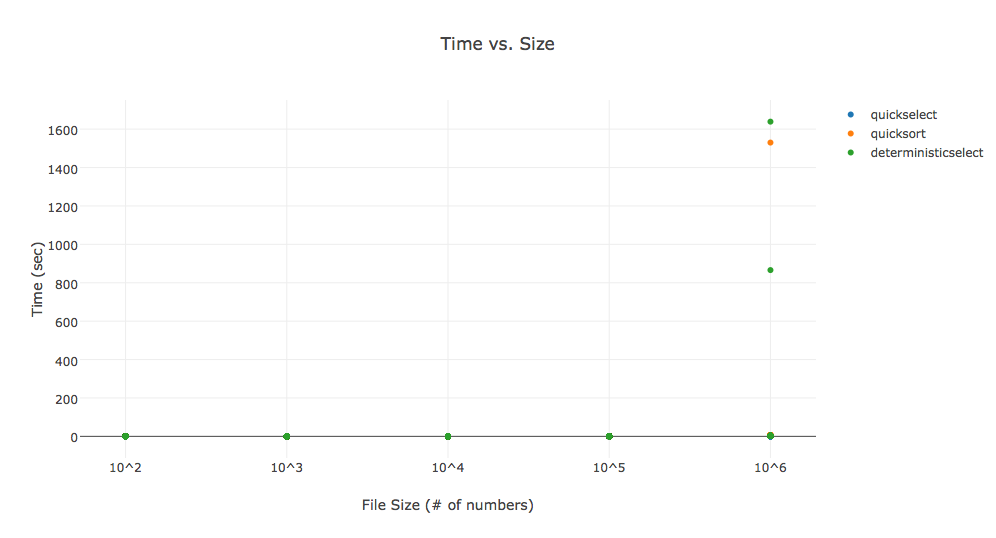
\includegraphics[scale=0.45]{resultsWoutliers}

Three outliers, two from deterministicselect and one from quicksort, clearly skewed our plot. We examined the lists that took substantially longer to complete to determine why; we discovered Russell's computer had shifted into sleep mode and resumed executing once awoken. We felt justified in excluding the outliers and recreated the previous plot to gain a better sense of each algorithm's performance.

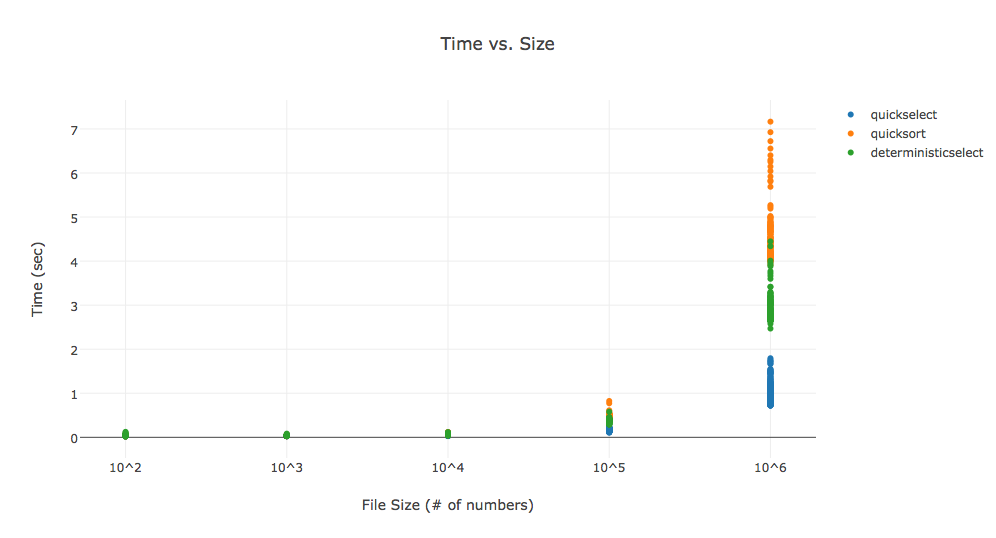
\includegraphics[scale=.45]{results}

To compare performance by list length, we plotted the performance of all three algorithms in a histogram for each of the five list lengths ($10^2, 10^3, 10^4, 10^5, 10^6$, respectively).

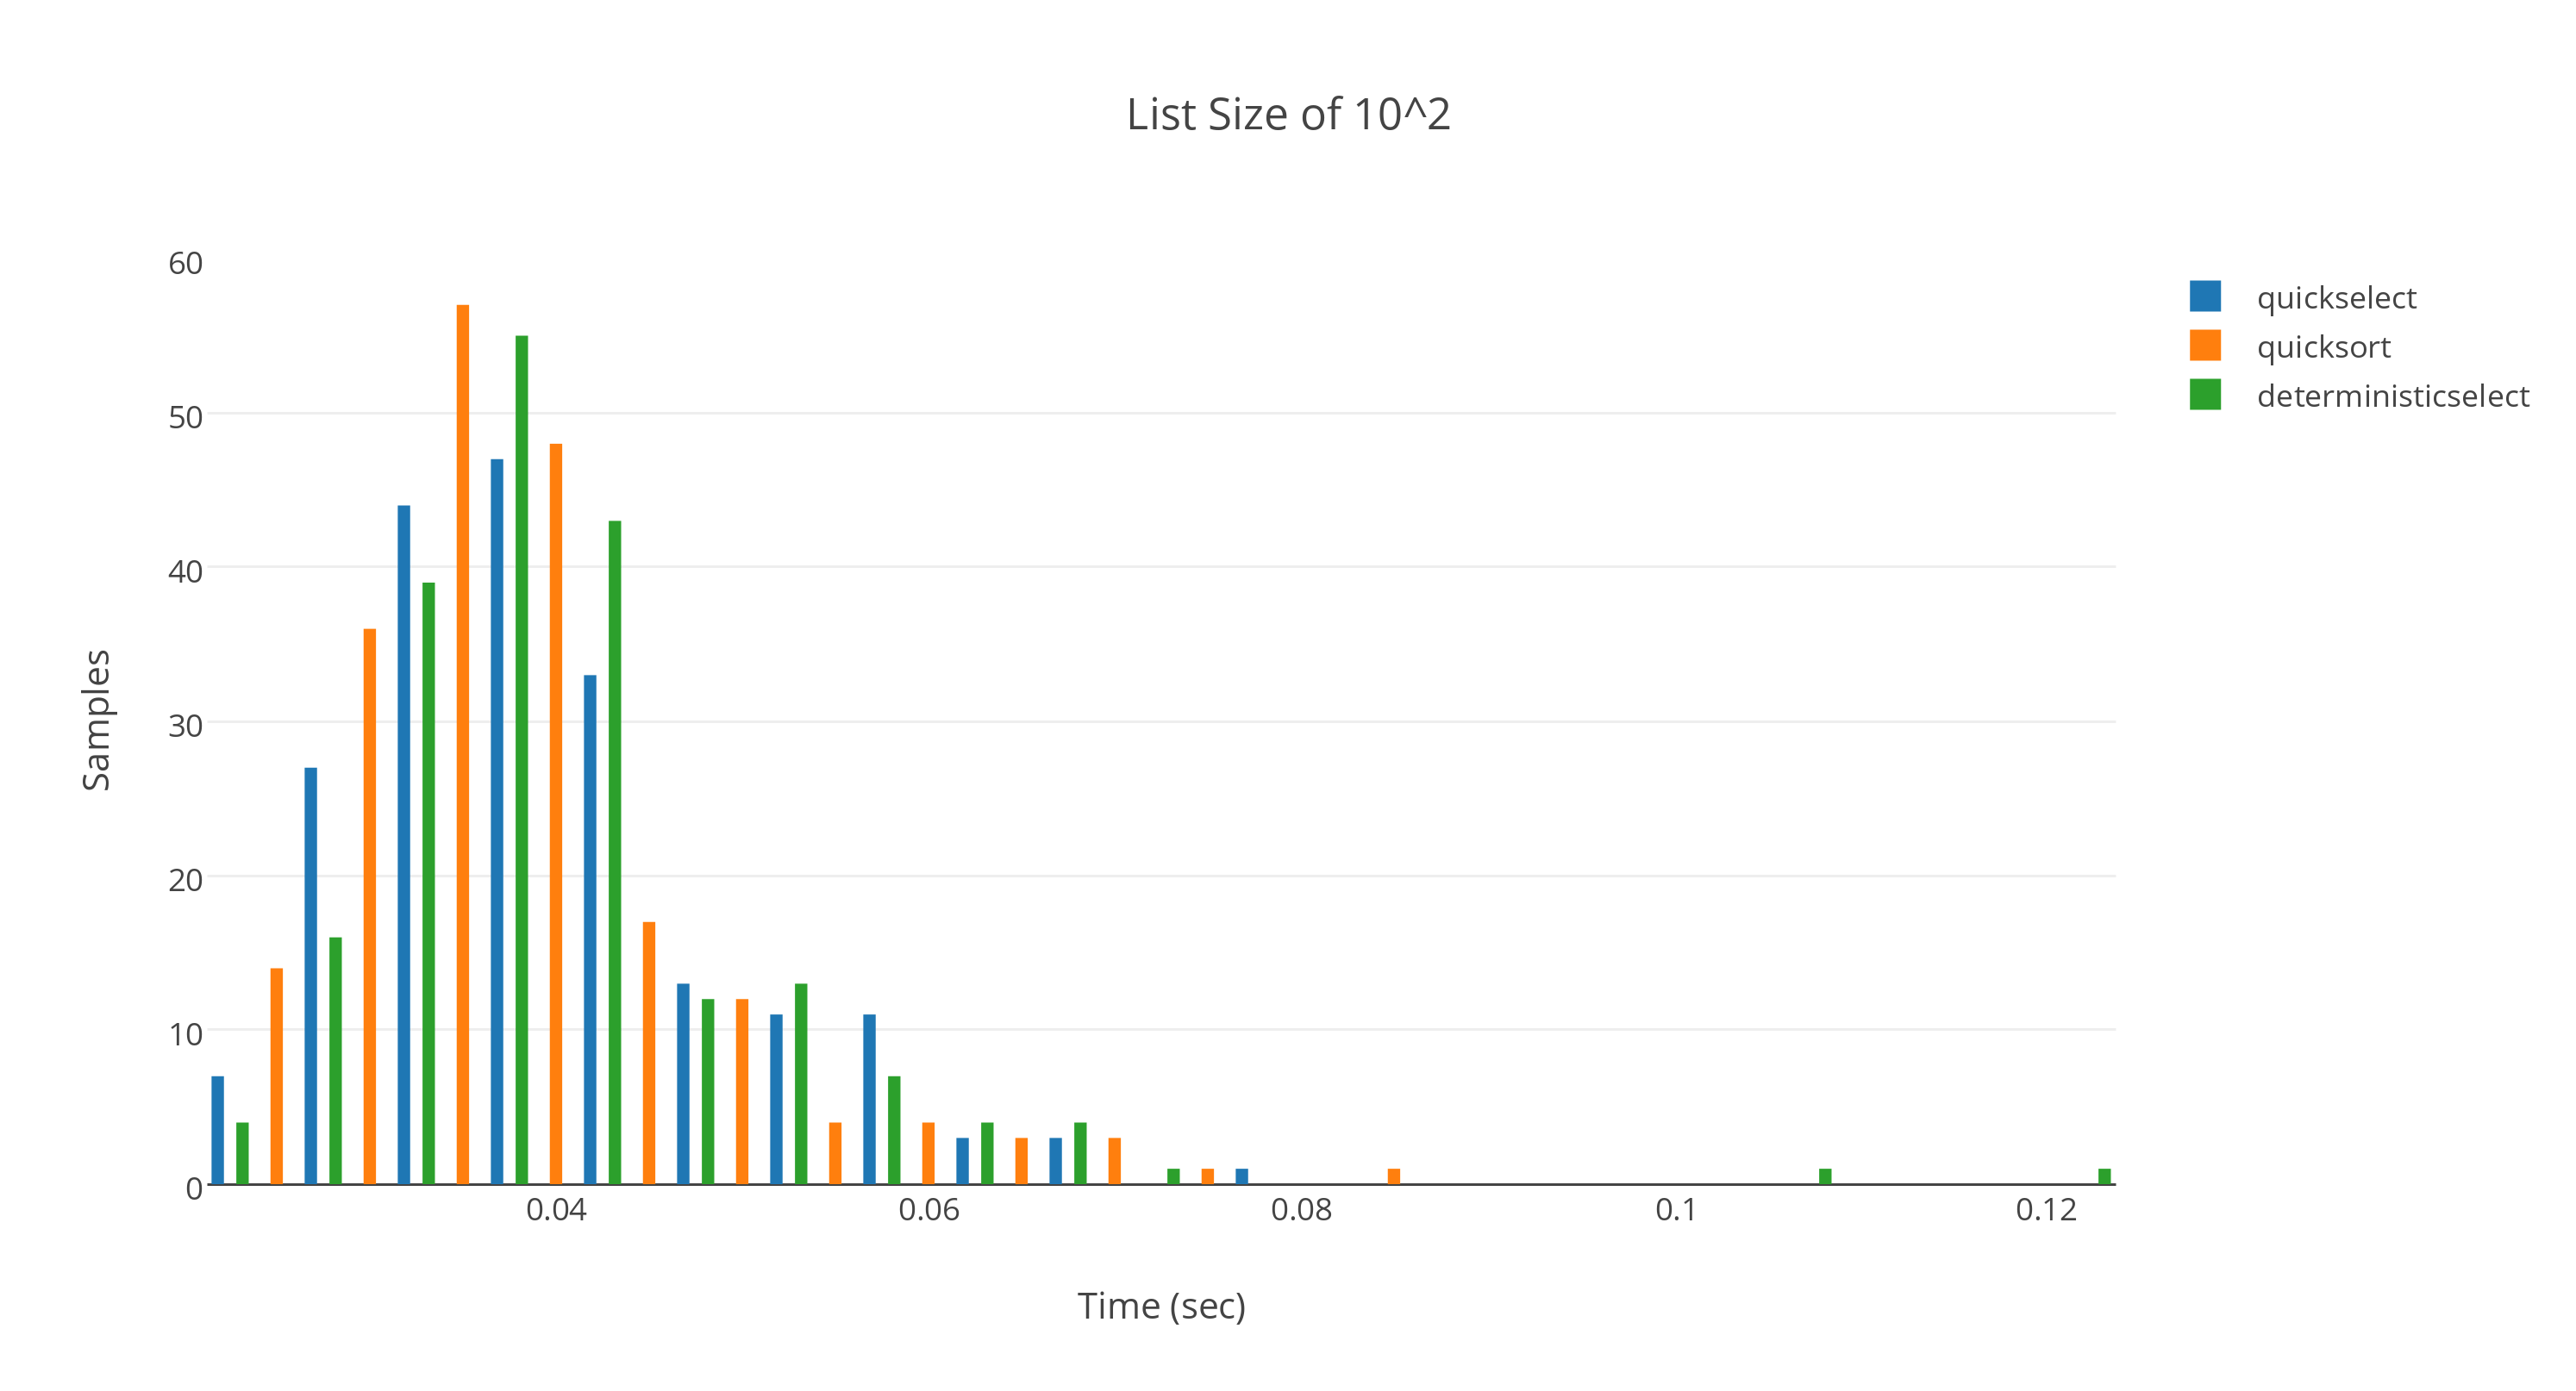
\includegraphics[scale=0.62]{list10^2}

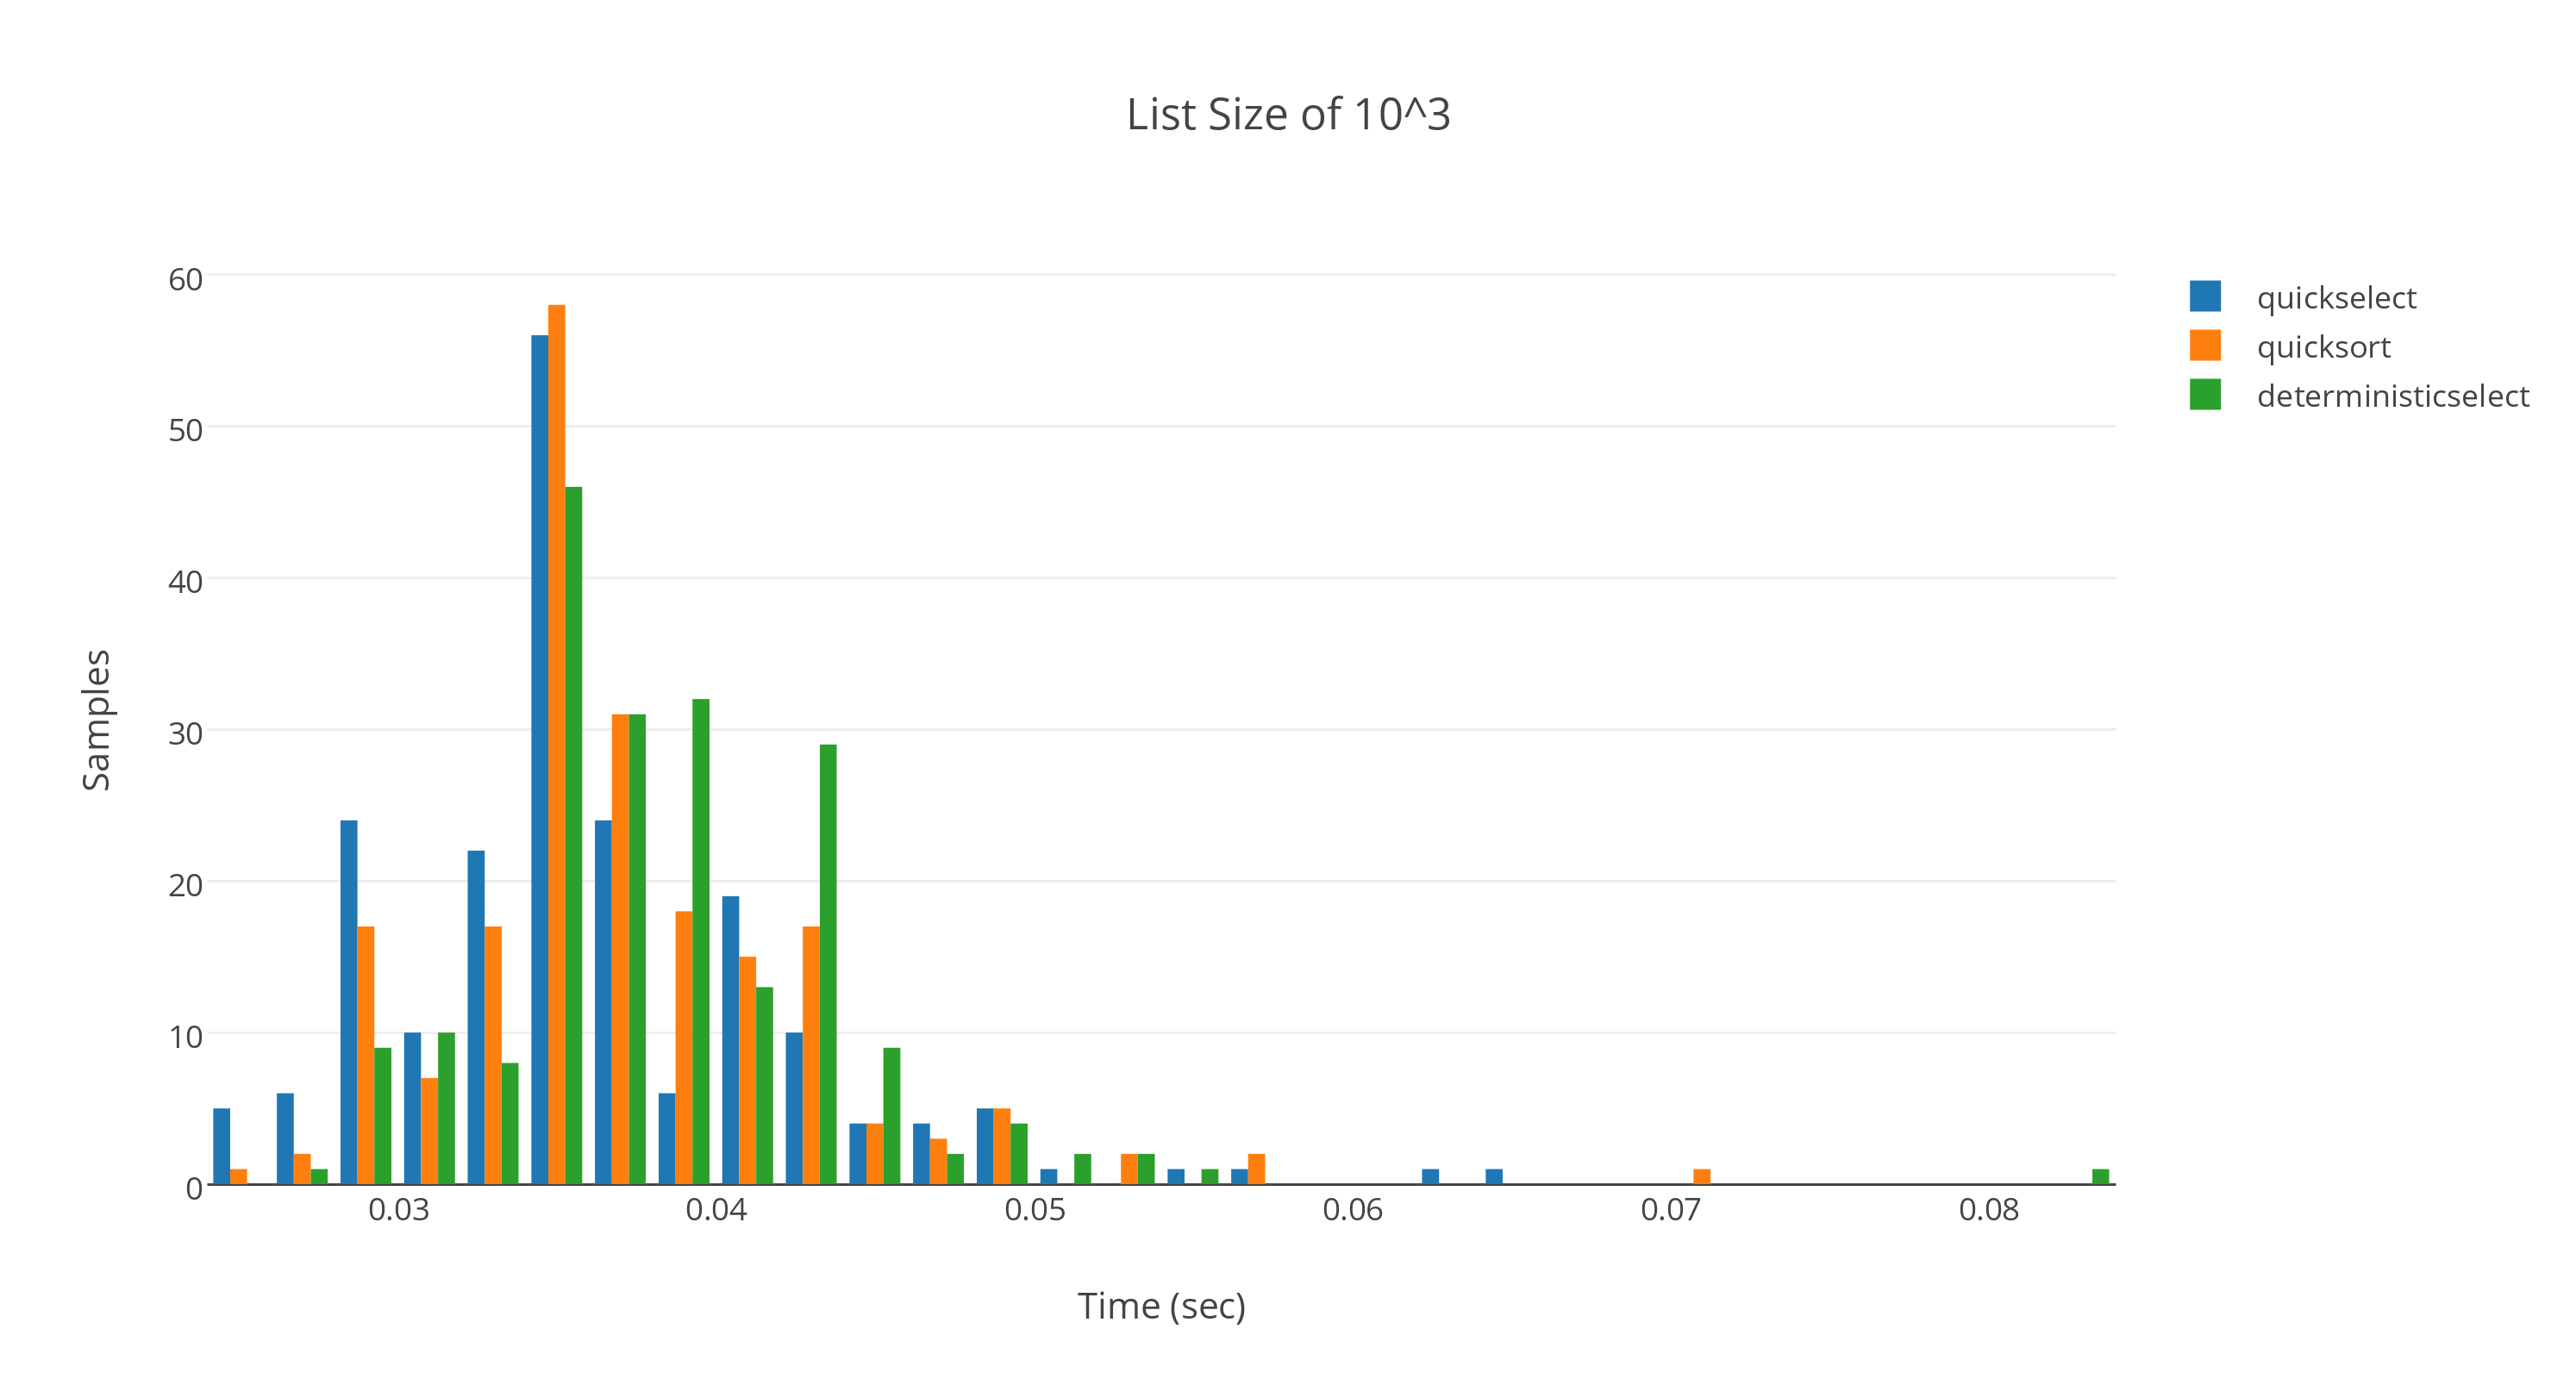
\includegraphics[scale=0.62]{list10^3}

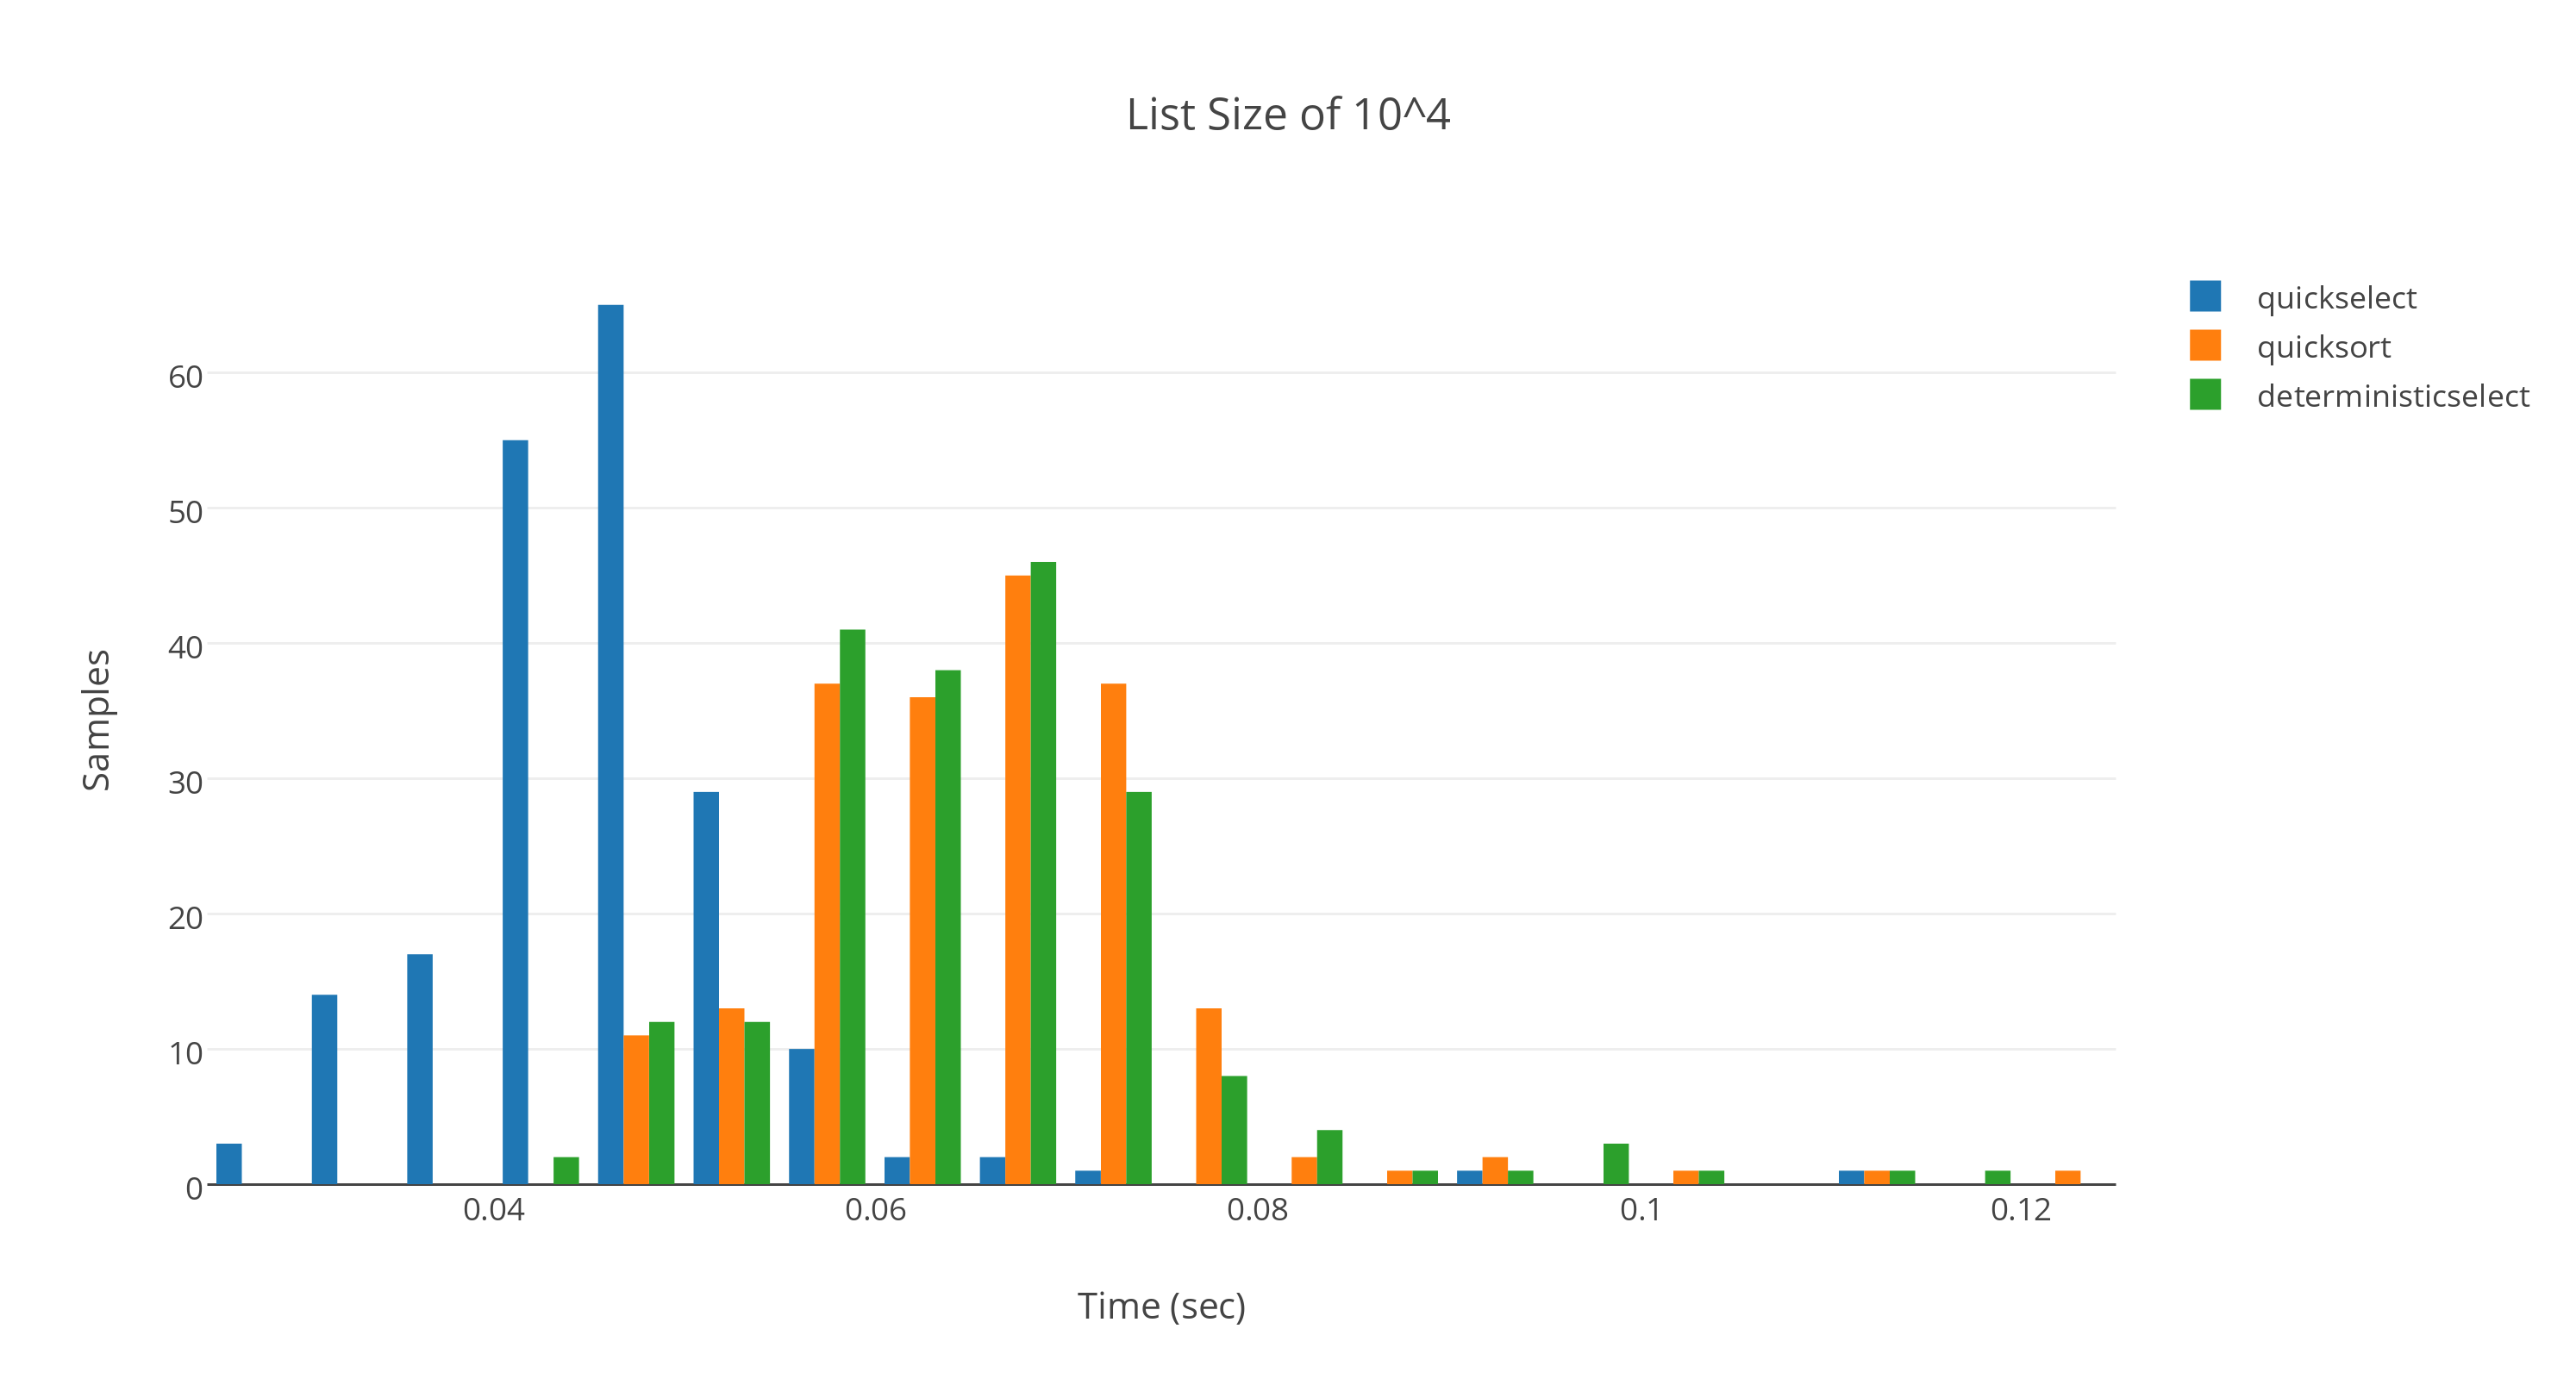
\includegraphics[scale=0.62]{list10^4}

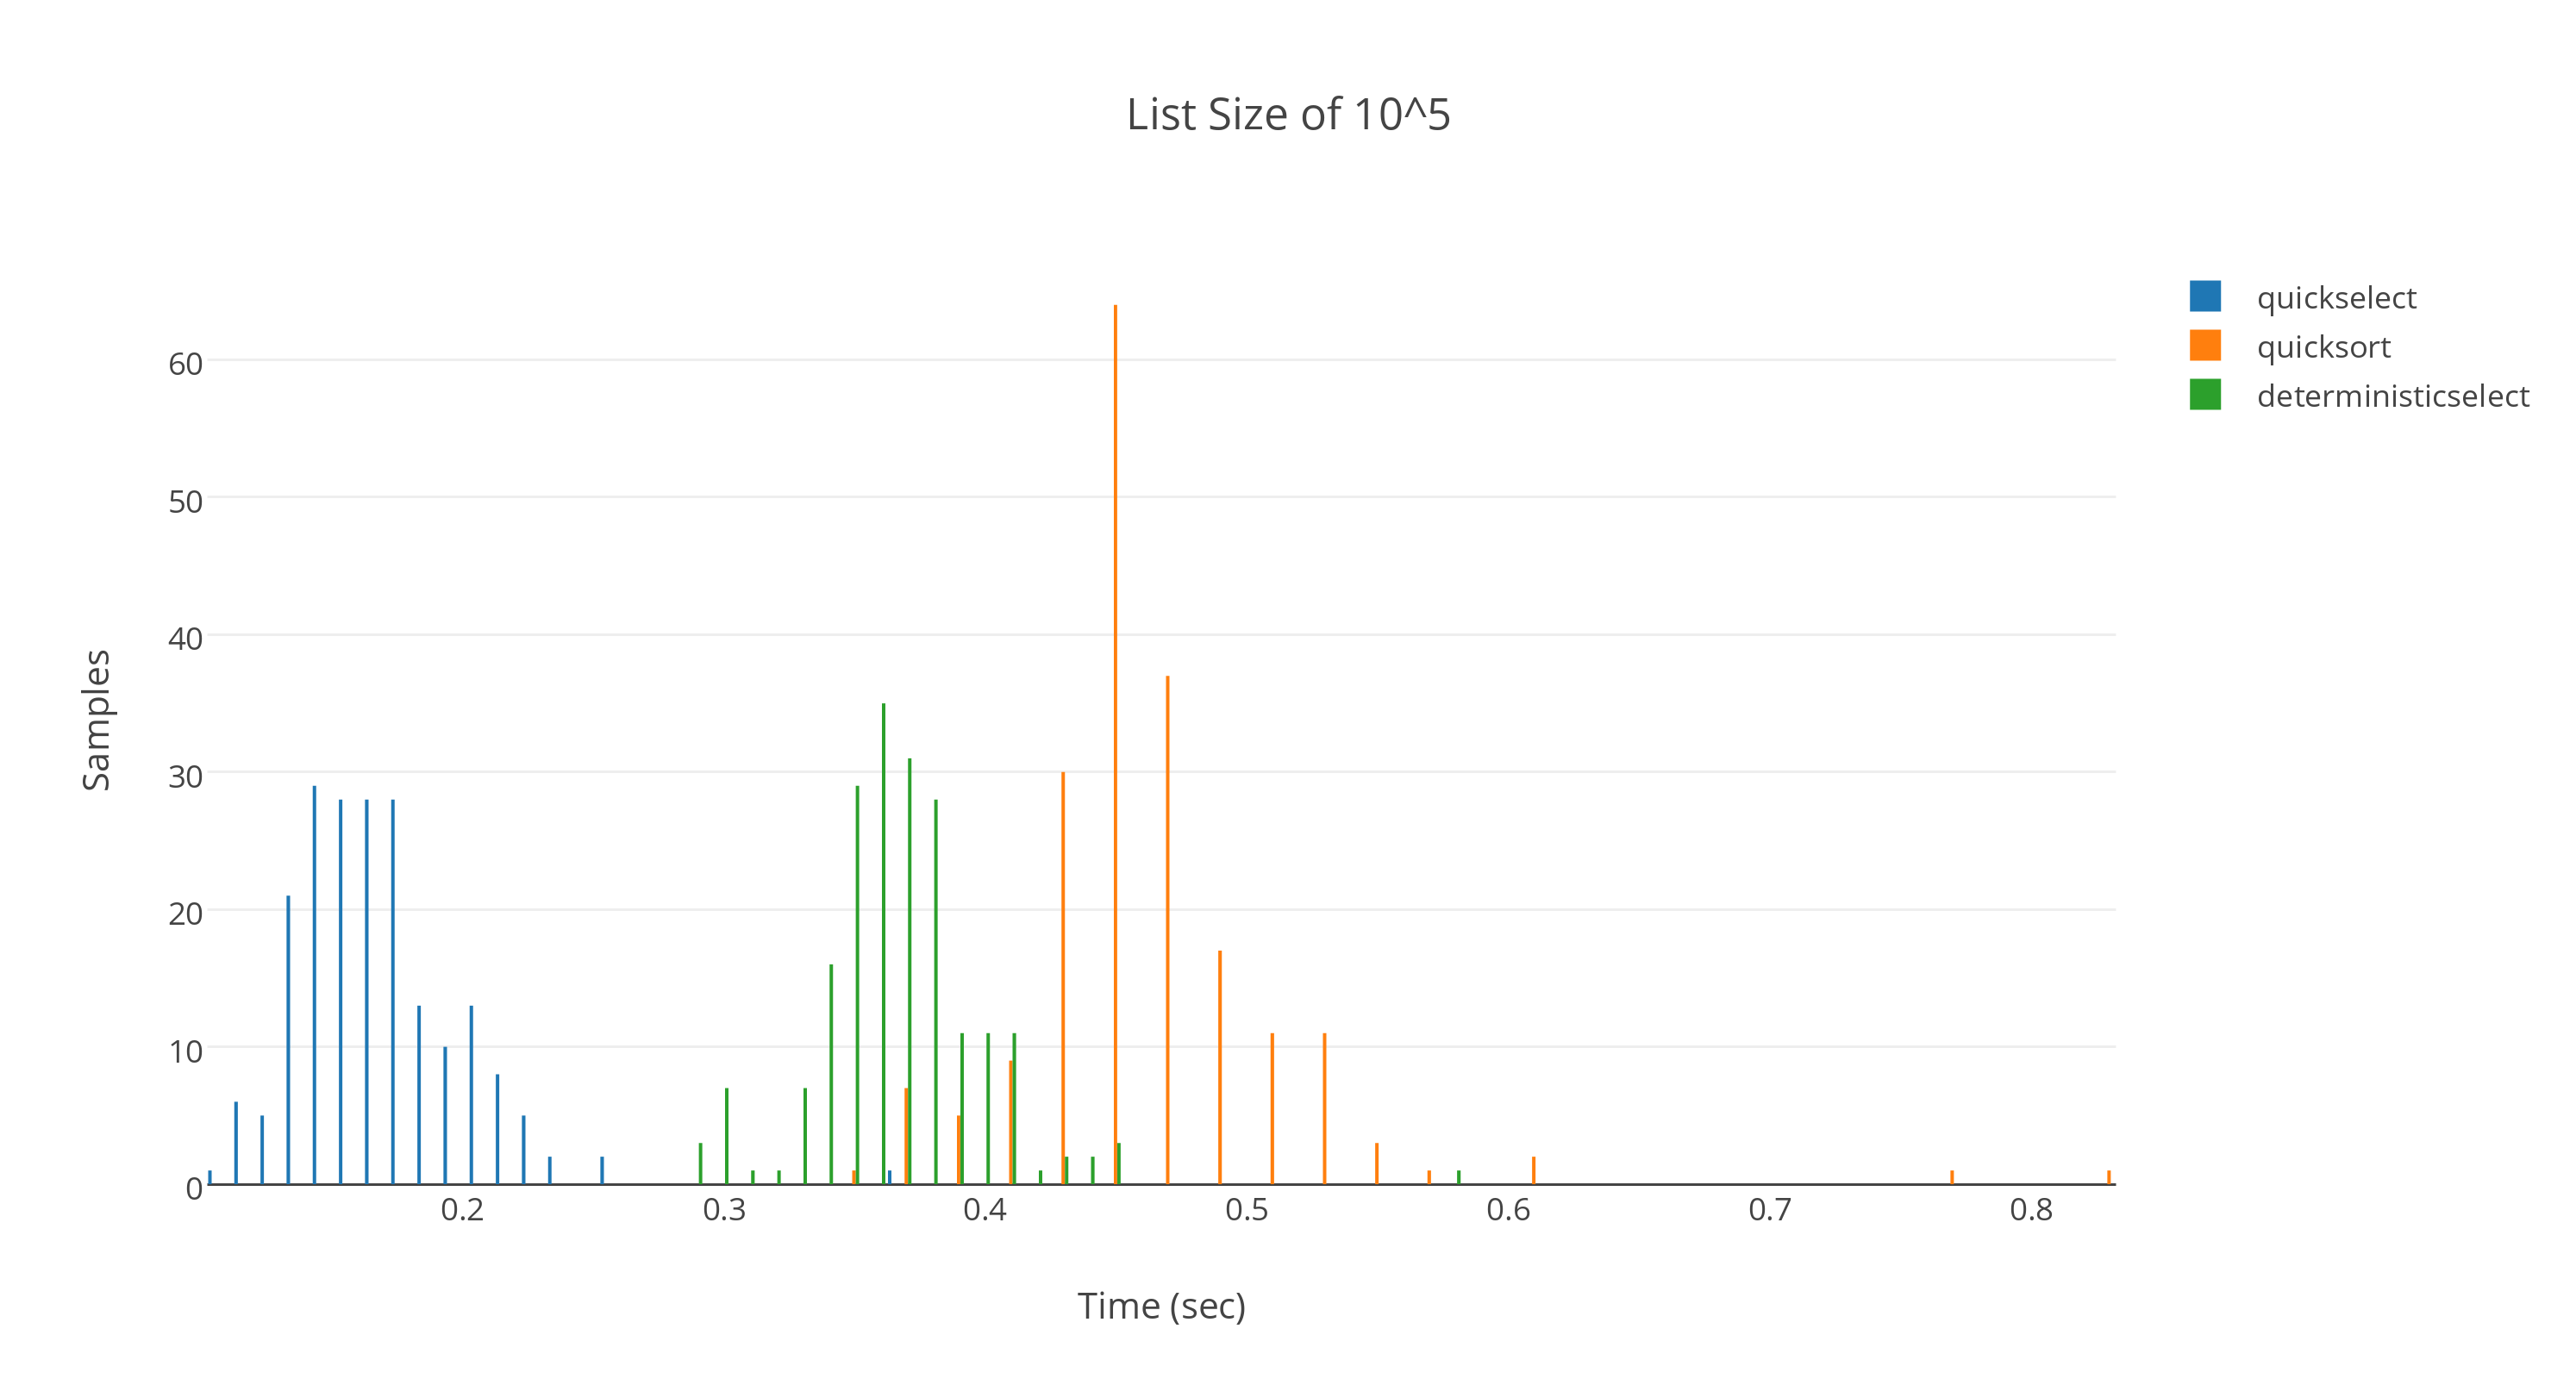
\includegraphics[scale=0.62]{list10^5}

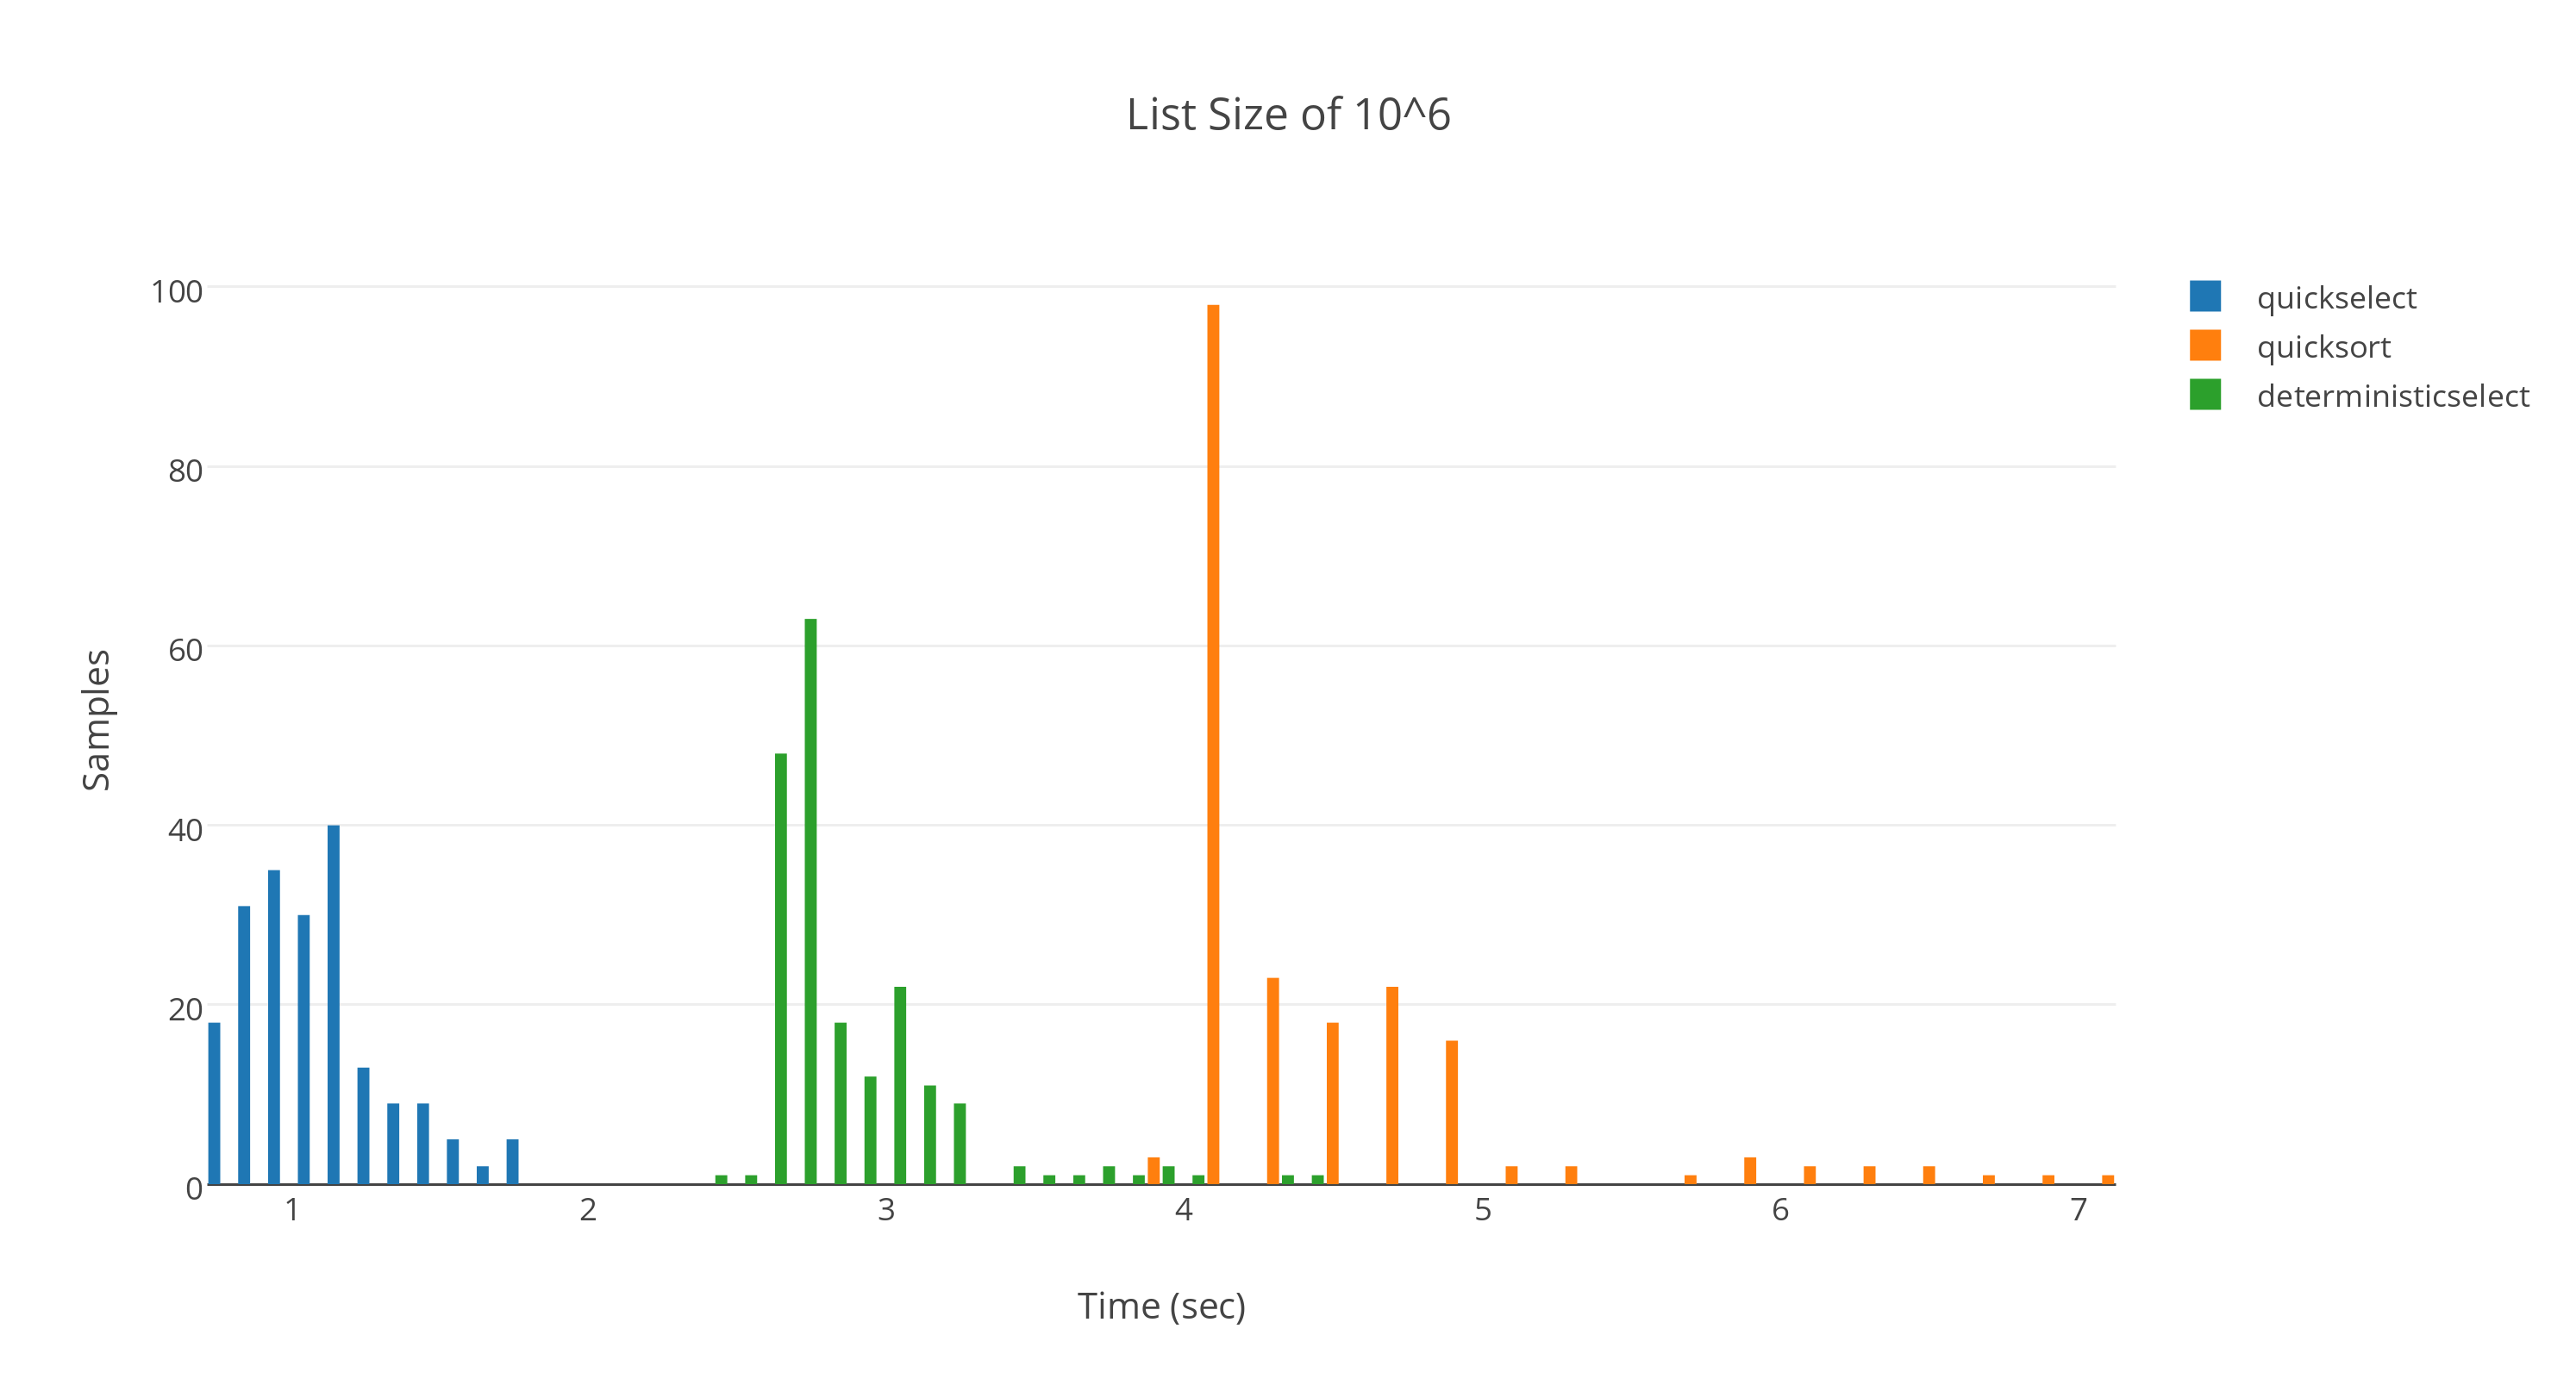
\includegraphics[scale=0.62]{list10^6}

As one can visually see, for short list lengths, the three algorithms perform the same. Quickselect begins to emerge as the leader as the list length reaches $10^4$ elements, with quicksort and deterministicselect still performing roughly the same. Once the list length reaches  $10^5$ elements, deterministicselect begins to pull ahead of quicksort, leaving clear performance differences between the three for lists of $10^6$ elements.

The puzzling question is why quickselect outperforms deterministicselect when deterministicselect has a guaranteed worst-case $O(n)$ runtime and quickselect only has a $O(n)$ runtime on average, with a worst-case runtime of $O(n^2)$. We believe the answer lies in the fact that the list elements are randomly generated. As a result, the selected pivot has a good chance of being near the median of the list. Since quickselect doesn't incur the costs of repeatedly determining the median in order to partition the list, quickselect outperforms deterministicselect.

\section*{Future Directions}
\indent \indent Given more time, there are three questions of interest we would have liked to pursue. First, at what list lengths do the performance of the three algorithms become statistically different? Second, quicksort has the advantage of sorting the entire list, making subsequent selections on the same list in constant time; supposing we wanted to make multiple selects on the same list, which algorithm would be best for which list lengths? Third, would the algorithms still have the same comparative performance over data that wasn't selected uniformly at random? We suspect that deterministicselect would overtake quickselect for non-random lists and could explore that through more sophisticated list generation techniques.

\section*{Conclusion}
\indent \indent Our goal was to compare the performance of three algorithms designed to select the $k$th smallest element of a list: quicksort, quickselect and deterministicselect. Quickselect was the fastest of the three, emerging as the clear winner for lists of length $10^4$ elements or more. Deterministicselect was roughly on par with quicksort up until lists of length $10^5$ or longer. These results did not agree with the theoretical analysis of the algorithms. We argued why the theoretical analysis produced a different conclusion than the empirical performance and suggested future directions of exploration.

\section*{Citations}
Quicksort. Wikipedia. Accessed June 6th, 2016. \url{https://en.wikipedia.org/wiki/Quicksort}\\

\noindent Quickselect. Wikipedia. Accessed June 6th, 2016. \url{https://en.wikipedia.org/wiki/Quickselect}\\

\noindent Median of Medians. Wikipedia. Accessed June 6th, 2016. \url{https://en.wikipedia.org/wiki/Median_of_medians}

\pagebreak

\section*{Pseudocode}

\subsection*{Quickselect Pseudocode}
Copied from Wikipedia article on Quickselect (see Citations):
\begin{lstlisting}
function quickselect(A, lo, hi)
    if lo < hi then
        p := partition(A, lo, hi)
        quicksort(A, lo, p)
        quicksort(A, p + 1, hi)
        
function partition(list, left, right, pivotIndex)
     pivotValue := list[pivotIndex]
     swap list[pivotIndex] and list[right]
     storeIndex := left
     for i from left to right-1
         if list[i] < pivotValue
             swap list[storeIndex] and list[i]
             increment storeIndex
     swap list[right] and list[storeIndex]
     return storeIndex
     
function select(list, left, right, n)
     loop
         if left = right
             return list[left]
         pivotIndex := (left + right) / 2
         pivotIndex := partition(list, left, right, pivotIndex)
         if n = pivotIndex
             return list[n]
         else if n < pivotIndex
             right := pivotIndex - 1
         else
             left := pivotIndex + 1
\end{lstlisting}

\subsection*{Deterministicselect Pseudocode}
Adapted from Wikipedia article on Median Of Medians (see Citations):

\begin{lstlisting}
function deterministicselect(list, left, right, n)
    loop
        if left = right
             return left
        pivotIndex := pivot(list, left, right)
        pivotIndex := partition(list, left, right, pivotIndex)
        if n = pivotIndex
            return n
        else if n < pivotIndex
            right := pivotIndex - 1
        else
            left := pivotIndex + 1
            
function partition(list, left, right, pivotIndex)
     pivotValue := list[pivotIndex]
     swap list[pivotIndex] and list[right]
     for i from left to right-1
         if list[i] < pivotValue
             swap list[storeIndex] and list[i]
             increment storeIndex
     swap list[right] and list[storeIndex]
     return storeIndex
     
function pivot(list, left, right)
     if right - left < 5:
         return partition5(list, left, right)
     for i from left to right in steps of 5
         subRight := i + 4
         if subRight > right:
             subRight := right

         median5 := partition5(list, i, subRight)
         swap list[median5] and list[left + floor((i - left)/5)]
     newRight = left + ceil((right - left) / 5) - 1
     newK = left + (right - left)/10
     return select(list, left, newRight, newK)
     
function partition5(list, left, right)
     return left + index of median of list[left:right]
\end{lstlisting}


\subsection*{Quicksort Pseudocode}
Copied from Wikipedia article on Quicksort (see Citations):

\begin{lstlisting}
function quicksort(A, lo, hi)
    if lo < hi then
        p := partition(A, lo, hi)
        quicksort(A, lo, p)
        quicksort(A, p + 1, hi)

function partition(A, lo, hi)
    pivot := A[lo]
    i := lo - 1
    j := hi + 1
    loop forever
        do
            i := i + 1
        while A[i] < pivot
        do
            j := j - 1
        while A[j] > pivot
        if i >= j then
            return j
        swap A[i] with A[j]
\end{lstlisting}

\end{document}
